\documentclass[aspectratio=169, table]{beamer}

\usepackage{array}
\usepackage{colortbl}
\usepackage{tabularx}
\usepackage{xcolor}
\usepackage{tikz}
\usetikzlibrary{arrows.meta, positioning, calc, fit}

\makeatletter
\def\input@path{{../theme/}}
\makeatother
\graphicspath{{../theme/}{../../figures/}}
\usetheme{Pradita}

\newcommand{\sectionframe}[1]{%
  \begin{frame}{\hfill}
    \centering
    \Huge{\textbf{#1}}
  \end{frame}
}

\newcommand{\takeaway}[1]{%
  \vspace{4pt}
  {\footnotesize #1}
}

\title{\huge Lapisan Teknologi\\
  \vspace{8pt}
  pada ArchiMate}
\subtitle{IT30713 - Enterprise \& Platform Architecture}
\author{\textbf{Alfa Yohannis}}
\date{11 Juli 2026}

\begin{document}

\frame{\titlepage}

\begin{frame}[fragile]
  \frametitle{Contents}
  \vspace{20pt}
  \begin{columns}[t]
    \column{0.5\textwidth}
    \tableofcontents[sections={1-4}]

    \column{0.5\textwidth}
    \tableofcontents[sections={5-8}]
  \end{columns}
\end{frame}

\begin{frame}{\hfill}
  \centering
  \Huge{\textbf{Perangkat lunak sudah dirancang---di atas apa ia berjalan?}}
\end{frame}

% ============================================================
\section{Orientasi Bab}
\sectionframe{Orientasi Bab}

\begin{frame}{Tujuan Pembelajaran}
  \vspace{6pt}
  \begin{itemize}
    \item Menjelaskan elemen \textbf{lapisan teknologi} ArchiMate: node, perangkat
          (\emph{device}), \emph{system software}, layanan teknologi, artefak, dan
          jaringan.
    \item Menyusun \textbf{arsitektur teknologi} acuan yang menggelar komponen
          aplikasi dan mewujudkan objek data.
    \item Menempatkan analisis dalam \textbf{TOGAF ADM Fase D (Teknologi)}:
          \emph{baseline}, \emph{target}, dan kesenjangan.
    \item Menutup rantai keterlacakan motivasi $\rightarrow$ \dots $\rightarrow$
          aplikasi $\rightarrow$ data $\rightarrow$ \textbf{teknologi}.
  \end{itemize}
  \takeaway{Arah sesi: dari ``perangkat lunak apa'' menuju ``di atas node \&
  artefak apa ia digelar''.}
\end{frame}

\begin{frame}{Ringkasan Awal Bab}
  \vspace{6pt}
  \begin{itemize}
    \item Lapisan teknologi menutup \textbf{Fase D}: \textbf{node menggelar}
          komponen aplikasi; \textbf{artefak mewujudkan} objek data.
    \item Elemen inti: \emph{node}, \emph{device}, \emph{system software},
          \emph{technology service}, \emph{artifact}, \emph{communication network}.
    \item Studi kasus berjalan: kluster kontainer, server basis data, dan sistem
          inti (\emph{mainframe}) untuk rel Transfer Dana.
    \item Keluaran bab memperkuat \textbf{Analisis} teknologi \& menjadi
          \textbf{kerangka akhir} makalah.
  \end{itemize}
  \takeaway{Di sinilah rantai keterlacakan tertutup: aplikasi \& data
  \emph{digelar} pada infrastruktur nyata.}
\end{frame}

% ============================================================
\section{Mengapa Lapisan Teknologi}
\sectionframe{Mengapa Lapisan Teknologi}

\begin{frame}{Posisi Lapisan Teknologi dalam ArchiMate}
  \vspace{2pt}
  \centering
  \scalebox{0.74}{
    \begin{tikzpicture}[
      font=\small\bfseries,
      node distance=2.2mm,
      layer/.style={draw, rounded corners=1.5mm, align=left, minimum width=82mm,
        minimum height=10mm, inner xsep=4mm},
      strat/.style={layer, fill=orange!16},
      biz/.style={layer, fill=praditagreen!22},
      app/.style={layer, fill=blue!16},
      tech/.style={layer, fill=praditagreen!30, draw=praditagreen, line width=0.6mm},
      impl/.style={layer, fill=orange!10},
    ]
      \node[strat] (s) {STRATEGI\\
        \footnotesize\mdseries Sumber daya, kapabilitas, arah tindakan};
      \node[biz, below=of s] (b) {BISNIS\\
        \footnotesize\mdseries Aktor, peran, proses, layanan, objek bisnis};
      \node[app, below=of b] (a) {APLIKASI\\
        \footnotesize\mdseries Komponen, layanan, fungsi, antarmuka, objek data};
      \node[tech, below=of a] (t) {TEKNOLOGI (\& FISIK) \quad$\leftarrow$ \emph{fokus sesi ini}\\
        \footnotesize\mdseries \textbf{Node, device, \emph{system software}, layanan,
        artefak, jaringan}};
      \node[impl, below=of t] (i) {IMPLEMENTASI \& MIGRASI\\
        \footnotesize\mdseries \emph{Work package}, \emph{deliverable}, \emph{gap}};
      \node[draw, rounded corners=2mm, fill=purple!22, align=center,
        text width=16mm, minimum height=60mm, right=5mm of a, font=\bfseries]
        (mot) {M\\O\\T\\I\\V\\A\\S\\I\\[2mm]\footnotesize\mdseries (mengapa)};
    \end{tikzpicture}
  }

  \takeaway{Node \emph{menggelar} komponen aplikasi; artefak \emph{mewujudkan}
  objek data. Dipetakan ke fase \textbf{D (Teknologi)} TOGAF ADM.}
\end{frame}

\begin{frame}{Pola Penggelaran: Node, Artefak, Komponen}
  \vspace{2pt}
  \centering
  \scalebox{1.0}{
    \begin{tikzpicture}[
      font=\footnotesize,
      app/.style={rectangle, rounded corners=1.5mm, draw=blue!70!black, fill=blue!12,
        thick, align=center, text width=32mm, minimum height=10mm},
      tech/.style={rectangle, rounded corners=1.5mm, draw=praditagreen,
        fill=praditagreen!18, thick, align=center, text width=32mm, minimum height=10mm},
      data/.style={rectangle, rounded corners=1.5mm, draw=cyan!60!black, fill=cyan!12,
        thick, align=center, text width=30mm, minimum height=10mm},
      link/.style={-Latex, thick, draw=gray!60}
    ]
      \node[app] (comp) {Komponen Aplikasi};
      \node[tech, below=11mm of comp] (node) {Node};
      \node[tech, right=22mm of node] (art) {Artifact};
      \node[data, below=11mm of art] (do) {Objek Data};
      \draw[link] (node) -- node[right,font=\scriptsize\bfseries]{menggelar} (comp);
      \draw[link] (node) -- node[above,font=\scriptsize\bfseries]{menggelar} (art);
      \draw[link, densely dashed] (art) -- node[right,font=\scriptsize\bfseries]{mewujudkan} (do);
    \end{tikzpicture}
  }

  \takeaway{Node tak ``menjadi'' komponen---ia menyediakan tempat komponen
  \emph{berjalan}; artefak adalah \emph{wujud fisik} yang dapat disimpan.}
\end{frame}

% ============================================================
\section{TOGAF ADM Fase D}
\sectionframe{TOGAF ADM Fase D:\\ Arsitektur Teknologi}

\begin{frame}{Siklus TOGAF ADM}
  \vspace{8pt}
  \begin{columns}[c]
    \column{0.4\textwidth}
    \centering
    \scalebox{0.85}{
      \begin{tikzpicture}[
        font=\footnotesize\bfseries,
        phase/.style={circle, draw=praditagreen, line width=0.4mm,
          fill=praditagreen!15, minimum size=11mm, inner sep=0pt},
        reqman/.style={circle, draw=blueColor, line width=0.4mm, fill=blueColor!15,
          minimum size=21mm, inner sep=1pt, align=center, font=\scriptsize\bfseries},
        prelim/.style={circle, draw=orange!80!black, line width=0.4mm,
          fill=orange!25, minimum size=13mm, inner sep=0pt, align=center,
          font=\scriptsize\bfseries},
        ring/.style={-Latex, draw=praditagreen!75, line width=0.4mm},
        spoke/.style={draw=blueColor!35, line width=0.25mm},
      ]
        \node[reqman] (rm) at (0,0) {Manajemen\\Requirements};
        \foreach \ang/\lab in {90/A, 45/B, 0/C, -45/D, -90/E, -135/F, 180/G, 135/H}
          \node[phase] (\lab) at (\ang:2.6cm) {\lab};
        \node[prelim] (P) at (90:4.1cm) {Prelim.};
        \foreach \lab in {A,B,C,D,E,F,G,H} \draw[spoke] (\lab) -- (rm);
        \foreach \a/\b in {A/B, B/C, C/D, D/E, E/F, F/G, G/H, H/A}
          \draw[ring] (\a) to[bend left=12] (\b);
        \draw[ring, draw=orange!80!black] (P) -- (A);
        \node[phase, fill=blue!45, line width=0.7mm] at (-45:2.6cm) {D};
      \end{tikzpicture}
    }
    \column{0.6\textwidth}
    {\footnotesize TOGAF (\emph{The Open Group Architecture Framework}); ADM
    (\emph{Architecture Development Method}).\par}
    \vspace{5pt}
    \footnotesize
    \begin{itemize}\setlength{\itemsep}{1.0pt}
      \item \textbf{Prelim.}---Persiapan \& prinsip
      \item \textbf{A}---Visi Arsitektur
      \item \textbf{B}---Arsitektur Bisnis
      \item \textbf{C}---Arsitektur Sistem Informasi (Data \& Aplikasi)
      \item \textbf{\textcolor{blue!70!black}{D---Arsitektur Teknologi}}
            $\leftarrow$ \emph{sesi ini}
      \item \textbf{E}---Peluang \& Solusi
      \item \textbf{F}---Perencanaan Migrasi
      \item \textbf{G}---Tata Kelola Implementasi
      \item \textbf{H}---Manajemen Perubahan Arsitektur
      \item \textbf{Manajemen Requirements}---di pusat
    \end{itemize}
  \end{columns}
\end{frame}

\begin{frame}{Fase D (Teknologi): Lima Langkah}
  \vspace{2pt}
  \footnotesize
  \begin{columns}[t]
    \column{0.5\textwidth}
    \textbf{Apa \& Mengapa}
    \begin{itemize}\setlength{\itemsep}{2.5pt}
      \item Fase D: infrastruktur yang \textbf{menggelar} komponen dan
            \textbf{mewujudkan} data.
      \item Menghasilkan arsitektur teknologi \textbf{baseline} \&
            \textbf{target}.
      \item Selisihnya = \textbf{analisis kesenjangan}.
    \end{itemize}
    \column{0.5\textwidth}
    \textbf{Lima Langkah}
    \begin{enumerate}\setlength{\itemsep}{2.5pt}
      \item Ruang lingkup \& prinsip teknologi.
      \item Arsitektur teknologi \textbf{baseline}.
      \item Arsitektur teknologi \textbf{target}.
      \item Analisis \textbf{kesenjangan}.
      \item Masukan ke Fase E/F (implementasi).
    \end{enumerate}
  \end{columns}
  \vspace{2pt}
  \takeaway{Keluaran: katalog teknologi, diagram penggelaran, dan matriks
  komponen--terhadap--teknologi.}
\end{frame}

% ============================================================
\section{Elemen Lapisan Teknologi}
\sectionframe{Elemen Lapisan Teknologi}

\begin{frame}{Jenis Elemen dan Simbolnya di Archi}
  \vspace{6pt}
  \begin{columns}[c]
    \column{0.56\textwidth}
    \centering
    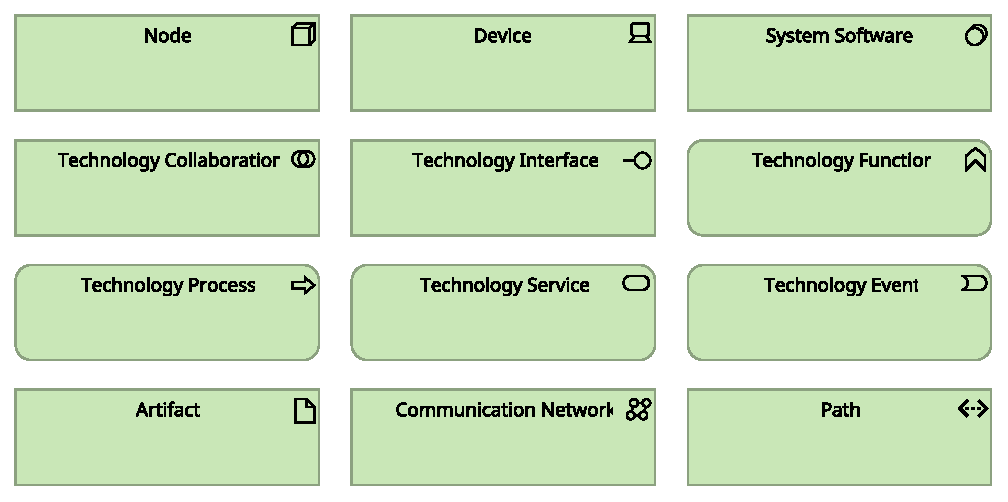
\includegraphics[width=\linewidth]{technology-legend.pdf}
    \column{0.44\textwidth}
    \footnotesize
    \begin{itemize}\setlength{\itemsep}{3pt}
      \item \textbf{Node} -- sumber daya komputasi.
      \item \textbf{Device} -- node fisik (perangkat keras).
      \item \textbf{System software} -- OS, runtime, DBMS.
      \item \textbf{Technology service} -- layanan node.
      \item \textbf{Artifact} -- wujud fisik data/komponen.
      \item \textbf{Communication network} -- penghubung node.
    \end{itemize}
  \end{columns}
  \takeaway{Elemen teknologi berwarna kehijauan; ikon pojok membedakan jenisnya.}
\end{frame}

\begin{frame}{Membedakan Elemen Teknologi}
  \vspace{6pt}
  \begin{itemize}
    \item \textbf{Node:} sumber daya komputasi yang menggelar perangkat
          lunak---``Kluster Kontainer'', ``Server Basis Data''.
    \item \textbf{Device:} node fisik---``Server Fisik (Data Center)''.
    \item \textbf{System software:} perangkat lunak sistem---``Runtime Kontainer
          \& OS'', ``PostgreSQL''.
    \item \textbf{Technology service:} layanan node ke aplikasi---``Layanan
          Komputasi Kontainer''.
    \item \textbf{Artifact:} wujud fisik yang dapat digelar---``Container Image'',
          ``Skema Basis Data''.
  \end{itemize}
  \takeaway{Node \emph{tersusun atas} device \& system software, \emph{mewujudkan}
  layanan teknologi, dan \emph{menggelar} artefak serta komponen.}
\end{frame}

\begin{frame}{}
  \centering
  \vspace{1mm}
  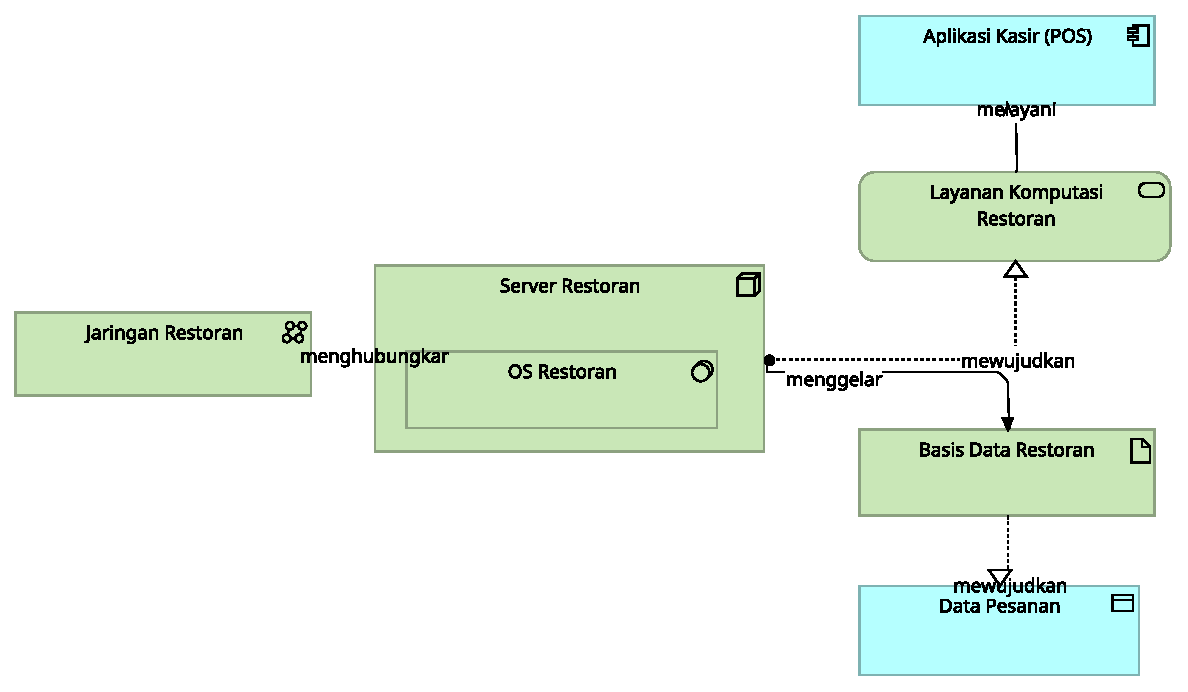
\includegraphics[width=\textwidth,height=.8\textheight,keepaspectratio]{technology-contoh.pdf}\\
  {\scriptsize Contoh interaksi antar-elemen teknologi (kasus restoran): node
  tersusun atas OS, mewujudkan layanan, menggelar aplikasi \& artefak; artefak
  mewujudkan data.}
\end{frame}

% ============================================================
\section{Studi Kasus: Teknologi di Archi}
\sectionframe{Studi Kasus:\\ Arsitektur Teknologi Transfer di Archi}

\begin{frame}{}
  \centering
  \vspace{1mm}
  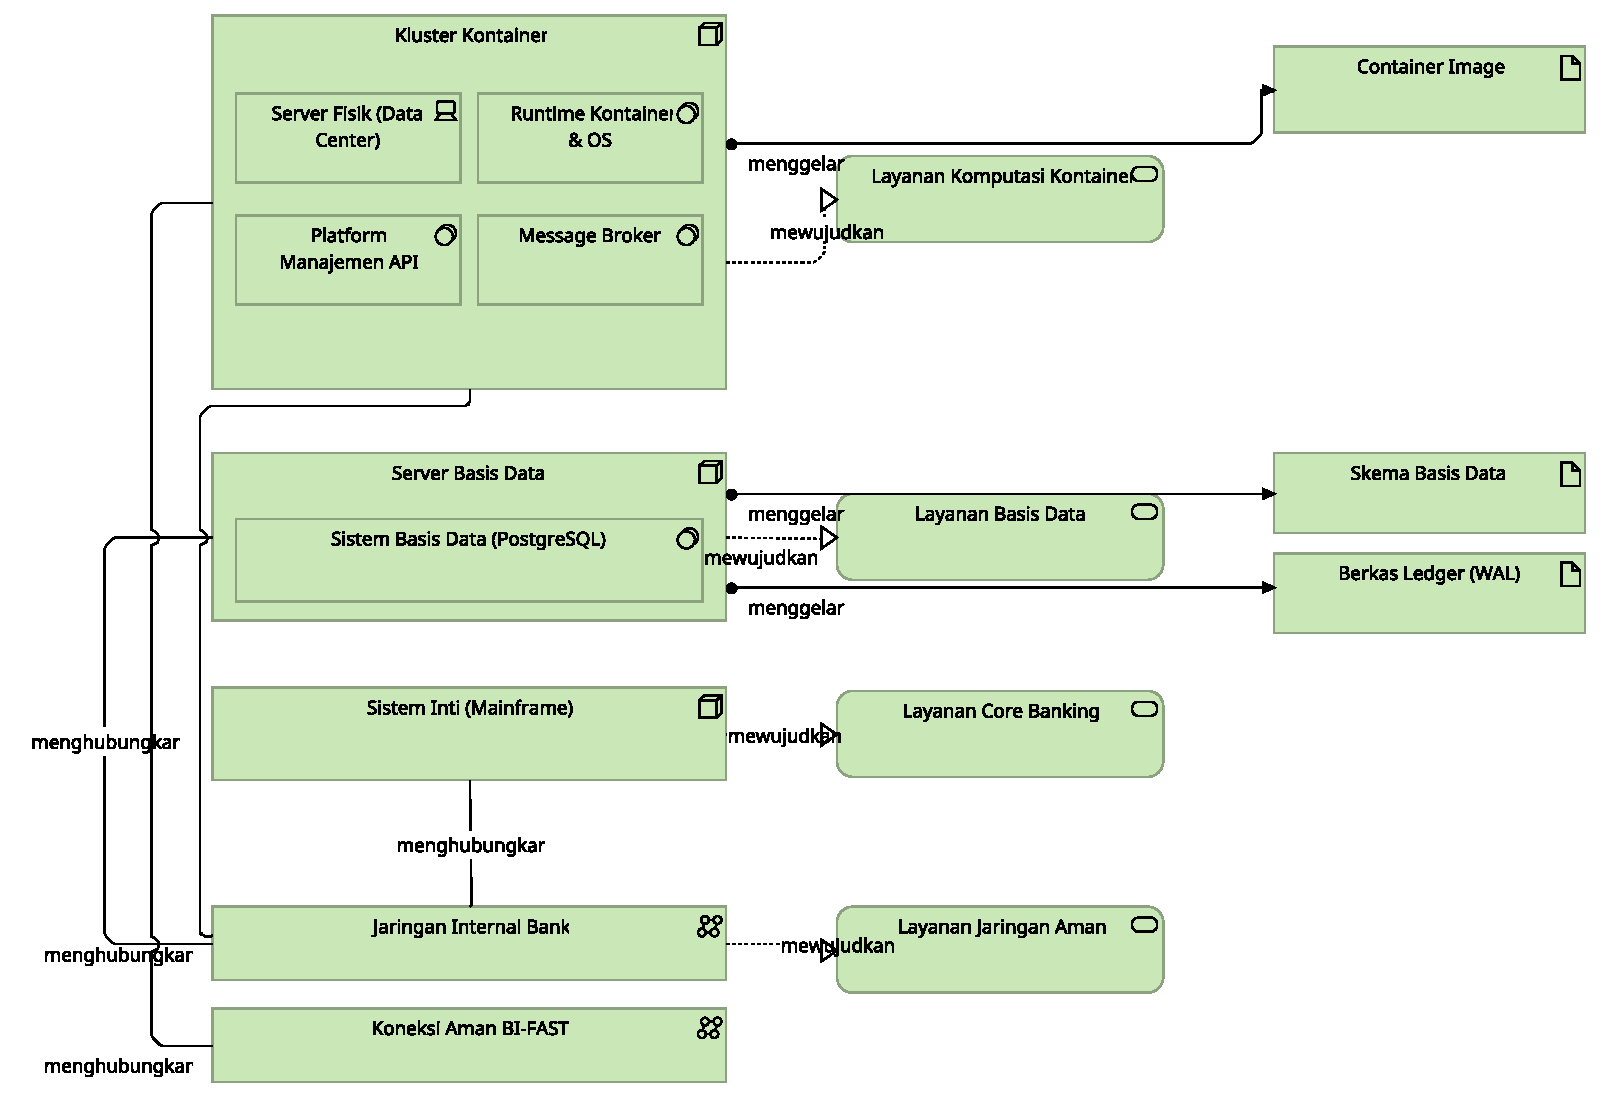
\includegraphics[width=\textwidth,height=.84\textheight,keepaspectratio]{technology-transfer.pdf}\\
  {\scriptsize Lanskap teknologi: node \emph{tersusun atas} perangkat \& system
  software, \emph{mewujudkan} layanan teknologi, \emph{menggelar} artefak, dan
  terhubung lewat \emph{jaringan}.}
\end{frame}

\begin{frame}{}
  \centering
  \vspace{1mm}
  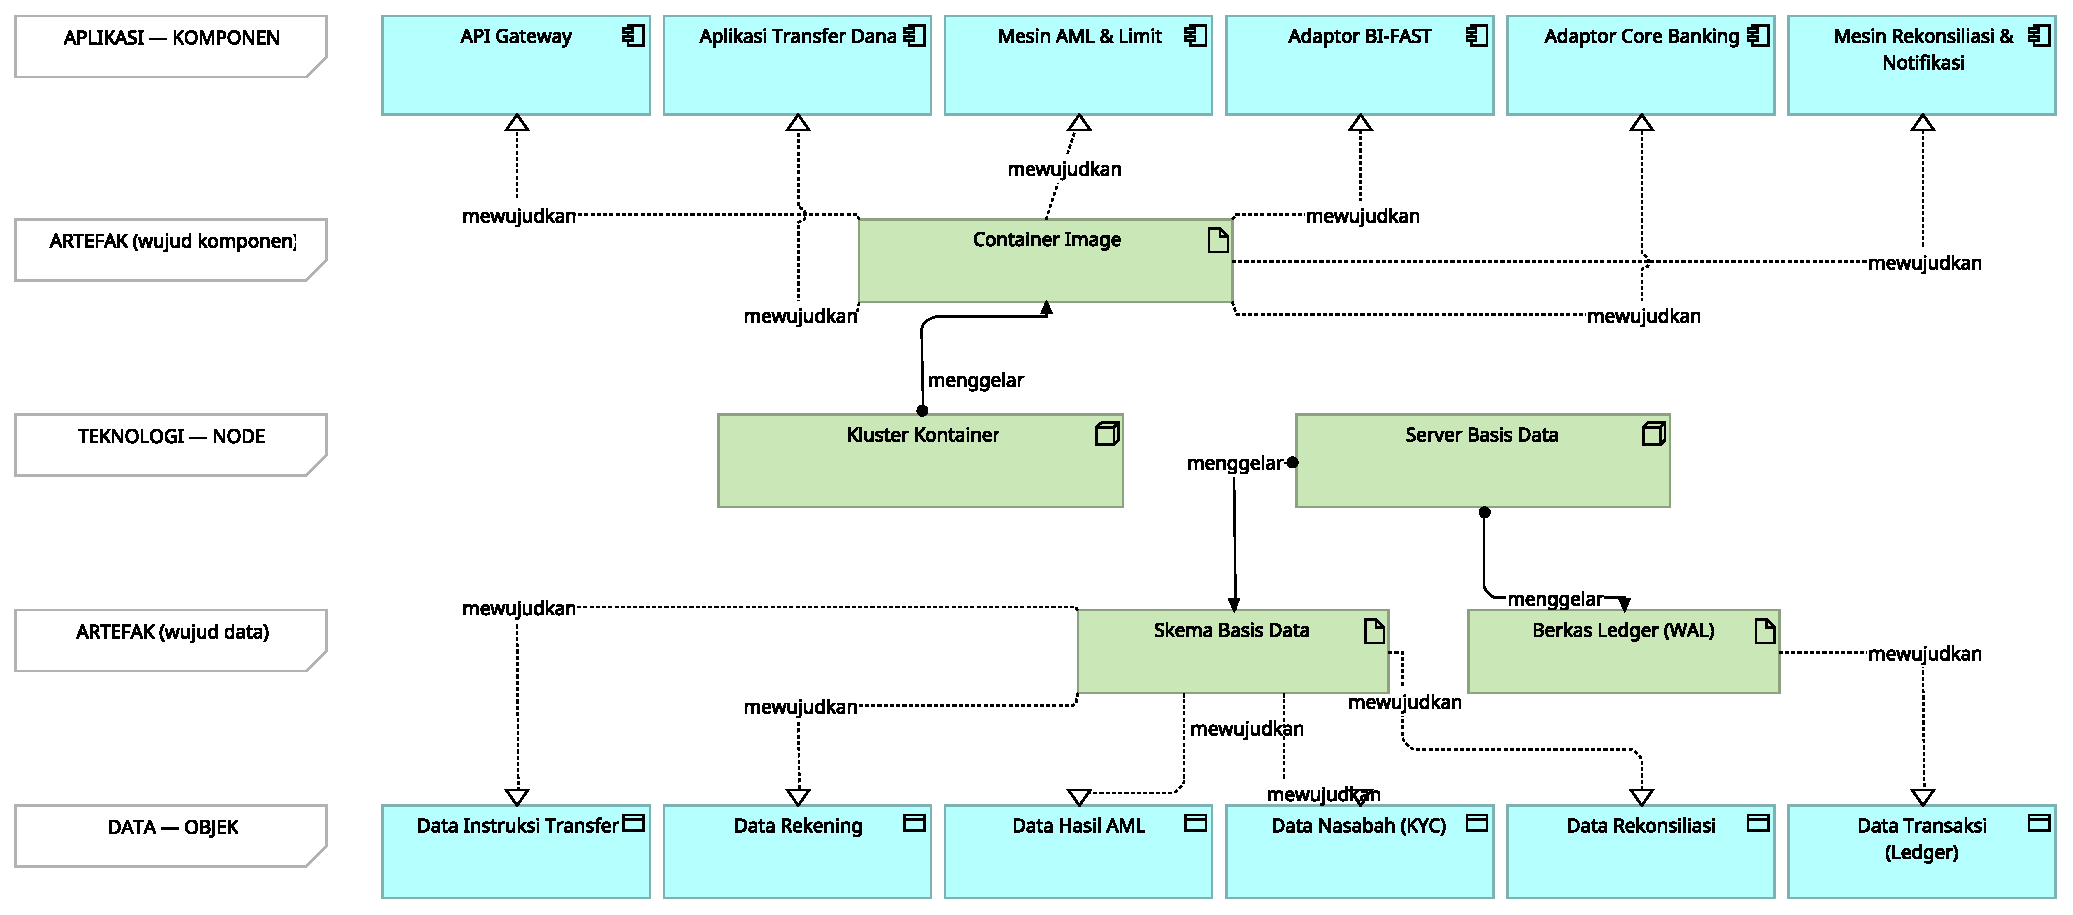
\includegraphics[width=\textwidth,height=.84\textheight,keepaspectratio]{technology-stack.pdf}\\
  {\scriptsize Penyelarasan \textbf{Aplikasi--Teknologi--Data}: node
  \emph{menggelar} komponen aplikasi; artefak \emph{mewujudkan} objek data,
  digelar di node basis data.}
\end{frame}

\begin{frame}{Cara Membaca: Rantai Lengkap Fase D}
  \vspace{4pt}
  \footnotesize
  \begin{itemize}\setlength{\itemsep}{2.5pt}
    \item \textbf{Komposisi:} node \emph{tersusun atas} device \& system
          software (ditunjukkan lewat pelingkupan).
    \item \textbf{Realisasi (node):} node \emph{mewujudkan} layanan teknologi.
    \item \textbf{Serving/Assignment:} node \emph{menggelar} komponen aplikasi.
    \item \textbf{Realisasi (artefak):} artefak \emph{mewujudkan} objek
          data---inilah jembatan teknologi ke data.
    \item \textbf{Asosiasi:} jaringan \emph{menghubungkan} node.
  \end{itemize}
  \takeaway{Rantai keterlacakan tertutup: komponen aplikasi $\rightarrow$ node;
  objek data $\rightarrow$ artefak $\rightarrow$ node.}
\end{frame}

% ============================================================
\section{Latihan dan Jembatan}
\sectionframe{Latihan dan Jembatan}

\begin{frame}{Latihan Terapan Individual}
  \vspace{8pt}
  \begin{itemize}
    \item \textbf{Latihan 8.1} -- Lanskap teknologi (node, system software,
          layanan, artefak, jaringan).
    \item \textbf{Latihan 8.2} -- Penyelarasan lintas-lapisan (aplikasi--teknologi
          --data) untuk satu kapabilitas.
    \item \textbf{Latihan 8.3} -- Pola penggelaran \& baseline--target.
    \item \textbf{Latihan 8.4} -- Paragraf analisis teknologi.
  \end{itemize}
  \takeaway{Semua latihan menjadi bahan langsung Analisis domain teknologi
  makalah.}
\end{frame}

\begin{frame}{Jembatan ke Bab Berikutnya}
  \vspace{8pt}
  \begin{itemize}
    \item Bab berikutnya beralih ke \textbf{lapisan implementasi \& migrasi}:
          \emph{work package}, \emph{deliverable}, \emph{plateau}, dan \emph{gap}.
    \item Seluruh artefak---motivasi, strategi, bisnis, data, aplikasi, dan
          teknologi---menjadi masukan peta jalan implementasi.
    \item Arsitektur teknologi target \& analisis kesenjangan langsung mengarah ke
          rencana bertahap.
  \end{itemize}
  \takeaway{Arsitektur teknologi yang jelas adalah fondasi bagi rencana
  implementasi yang realistis.}
\end{frame}

\begin{frame}{\hfill}
  \centering
  \Huge{\textbf{Terima kasih}}\\[8pt]
  \normalsize Pertanyaan \& diskusi
\end{frame}

\end{document}
